\section{Joint Segmentation and Tracking}

\begin{frame}{Motivation}
    \begin{figure}
    \centering
    \begin{subfigure}[t]{0.48\textwidth}
        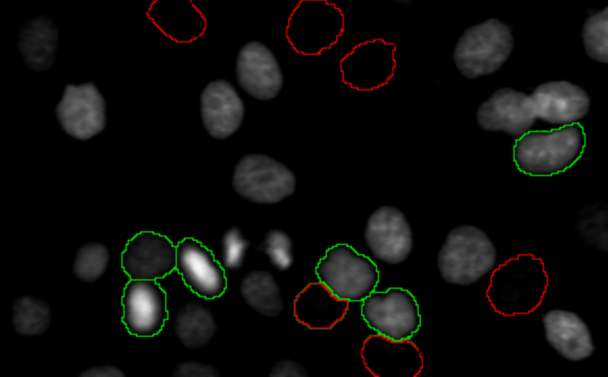
\includegraphics[width=\textwidth]{images/joint/mitocheck_255_max.pdf}
        \caption{}
        \label{fig:joint-underseg-no-detection}
    \end{subfigure}
    \hfill
    \begin{subfigure}[t]{0.48\textwidth}
        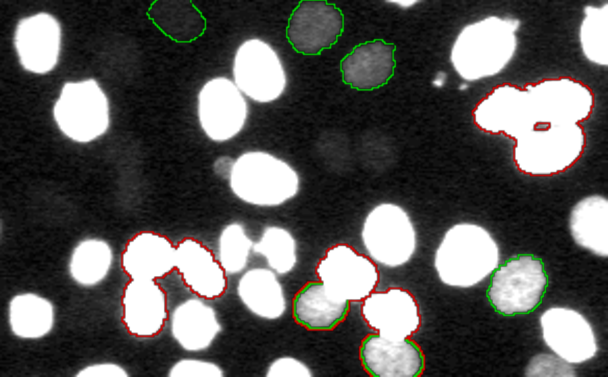
\includegraphics[width=\textwidth]{images/joint/mitocheck_030_max.pdf}
        \caption{}
        \label{fig:joint-underseg-mergers}
    \end{subfigure}
    \caption{Motivating the joint segmentation and tracking method.}
    \label{fig:joint-motivation-example}
\end{figure}
\end{frame}

\begin{frame}
    \frametitle{Workflow}
    \begin{figure}
        \centering
        \scalebox{0.65}{
            \begin{tikzpicture}
    \newcommand{\distancebetween}{20}
    \newcommand{\shiftdistance}{100}
    \newcommand{\scalingfactor}{0.12}
    \newcommand{\halfscalingfactor}{\scalingfactor}
    
    \begin{scope}
        \begin{scope}[baseline=(raw2)]
    \begin{scope}[yshift=\distancebetween,
        every node/.append style={yslant=0.5,xslant=-1},
        yslant=0.5,xslant=-1]
        \node[inner sep=0, label={[xshift=5]above:{}}] (raw1) {
            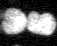
\includegraphics[width=\scalingfactor\textwidth]{images/joint/78_raw_crop_enhanced.png}
        };
    \end{scope}
    \begin{scope}[every node/.append style={yslant=0.5,xslant=-1},yslant=0.5,xslant=-1]
        \begin{pgfonlayer}{bglower}
            \node[inner sep=0, label={[xshift=15]above:{}}] (raw2) {
                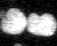
\includegraphics[width=\scalingfactor\textwidth]{images/joint/79_raw_crop_enhanced.png}
            };
        \end{pgfonlayer}
    \end{scope}
    \coordinate (base1) at (raw2.north west |- raw2.south west);
    \coordinate (base2) at (raw2.south east |- raw2.south west);
    % \draw [pllbl]
    % (base1) -- (base2) node[black,midway,yshift=-0.6cm]
    % {Raw Data};
    \path let \p1 = (base1.west), \p2 = (base2.east) in
    node[pllbltxt, minimum width=\x2-\x1] (labelraw) at ($(base1)!0.5!(base2)$)
    {\phantom{g}Raw Data\phantom{g}};
    \begin{pgfonlayer}{bglower}
        \path[threed] (raw2.south east) -- (raw1.south east);
        \path[threed] (raw2.north east) -- (raw1.north east);
        \path[threed] (raw2.south west) -- (raw1.south west);
        \path[threed] (raw2.north west) -- (raw1.north west);
    \end{pgfonlayer}
\end{scope}

%%% Local Variables: 
%%% mode: latex
%%% TeX-master: "../../../main"
%%% End: 

        % \node[ultra thick, left=of raw1,yshift=5mm] {$t\phantom{+1}$};
        % \node[ultra thick, left=of raw2,yshift=5mm] {$t+1$};
        \begin{scope}[xshift=\shiftdistance, baseline=(seg2)]
    \begin{scope}[yshift=\distancebetween,
        every node/.append style={yslant=0.5,xslant=-1},
        yslant=0.5,xslant=-1]
        \node[inner sep=0, label={[xshift=5]above:{}}] (seg1) {
            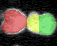
\includegraphics[width=\scalingfactor\textwidth]{images/joint/78_seg_crop.png}
        };
    \end{scope}
    \begin{scope}[every node/.append style={yslant=0.5,xslant=-1},yslant=0.5,xslant=-1]
        \begin{pgfonlayer}{bglower}
            \node[inner sep=0, label={[xshift=15]above:{}}] (seg2) {
                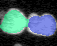
\includegraphics[width=\scalingfactor\textwidth]{images/joint/79_seg_crop.png}
            };
        \end{pgfonlayer}
    \end{scope}
    \coordinate (base1) at (seg2.north west |- seg2.south west);
    \coordinate (base2) at (seg2.south east |- seg2.south west);
    % \draw [pllbl]
    % (base1) -- (base2) node[black,midway,yshift=-0.6cm]
    % {Initial Oversegmentation};
    \path let \p1 = (base1.west), \p2 = (base2.east) in
    node[pllbltxt, minimum width=\x2-\x1] (labelseg) at ($(base1)!0.5!(base2)$) {Oversegmentation};
    \begin{pgfonlayer}{bglower}
        \path[threed] (seg2.south east) -- (seg1.south east);
        \path[threed] (seg2.north east) -- (seg1.north east);
        \path[threed] (seg2.south west) -- (seg1.south west);
        \path[threed] (seg2.north west) -- (seg1.north west);
    \end{pgfonlayer}
\end{scope}

%%% Local Variables: 
%%% mode: latex
%%% TeX-master: "../../../main"
%%% End: 

        \begin{scope}[xshift=2*\shiftdistance, baseline=(cc2)]
    \begin{scope}[yshift=\distancebetween,
        every node/.append style={yslant=0.5,xslant=-1},
        yslant=0.5,xslant=-1]
        \node[inner sep=0, label={[xshift=5]above:{}}] (merge1) {
            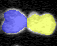
\includegraphics[width=\halfscalingfactor\textwidth]{images/joint/78_merge_crop.png}
        };
        \node[inner sep=0,xshift=47,yshift=-47, label={[xshift=5]above:{}}] (cc1) {
            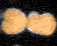
\includegraphics[width=\halfscalingfactor\textwidth]{images/joint/78_cc_crop.png}
        };
    \end{scope}
    \begin{scope}[every node/.append style={yslant=0.5,xslant=-1},yslant=0.5,xslant=-1]
        \begin{pgfonlayer}{bglower}
            \node[inner sep=0, label={[xshift=15]above:{}},rectangle,thin,draw] (merge2) {
                \phantom{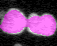
\includegraphics[width=\scalingfactor\textwidth]{images/joint/79_cc_crop.png}}
            };
            \node[xshift=47,yshift=-47,inner sep=0, label={[xshift=15]above:{}}] (cc2) {
                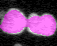
\includegraphics[width=\scalingfactor\textwidth]{images/joint/79_cc_crop.png}
            };
        \end{pgfonlayer}
    \end{scope}
    \coordinate (base1) at (merge1.north west |- cc2.south west);
    \coordinate (base2) at (cc1.south east |- cc2.south west);
    % \draw [pllbl]
    % (base1) -- (base2) node[black,midway,yshift=-0.6cm]
    % {Region Merging};
    \path let \p1 = (base1.west), \p2 = (base2.east) in
    node[pllbltxt, minimum width=\x2-\x1] (labelmerging) at ($(base1)!0.5!(base2)$) {Region Merging};
    \begin{pgfonlayer}{bglower}
        \path[threed] (merge2.south east) -- (merge1.south east);
        \path[threed] (merge2.north east) -- (merge1.north east);
        \path[threed] (merge2.south west) -- (merge1.south west);
        \path[threed] (merge2.north west) -- (merge1.north west);

        \path[threed] (cc2.south east) -- (cc1.south east);
        \path[threed] (cc2.north east) -- (cc1.north east);
        \path[threed] (cc2.south west) -- (cc1.south west);
        \path[threed] (cc2.north west) -- (cc1.north west);
    \end{pgfonlayer}
\end{scope}

%%% Local Variables: 
%%% mode: latex
%%% TeX-master: "../../../main"
%%% End: 

        \begin{pgfonlayer}{background}
            \node[plbg, fit=(raw2.south west) (raw2.north west)
            (raw1.north east) (cc1.south east) (labelraw)] (bg1) {};
        \end{pgfonlayer}
        \draw[arrows=->, ultra thick, transform canvas={xshift=-15}] (bg1.north west) -- (bg1.south
        west) node[midway, xshift=-7] (t1) {\large{$t$}};
    \end{scope}
    \begin{scope}[yshift=-7.5*\distancebetween, xshift=100]
        \begin{scope}
    \begin{scope}[yshift=1.5*\distancebetween,
        every node/.append style={yslant=0.5,xslant=-1},
        yslant=0.5,xslant=-1]
        \node[inner sep=0] (image1) {
            \phantom{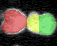
\includegraphics[width=\scalingfactor\textwidth]{images/joint/78_seg_crop.png}}
        };
        \begin{pgfonlayer}{upper}
            \begin{scope}[every node/.append style={scale=0.7}]
                \node[fg_det, label={[font=\tiny]center:$X_1^t$}] (a1) at (image1.south east) {};
                \node[fg_det, label={[font=\tiny]center:$X_2^t$}] (a2) at ($(image1.south east)!0.5!(image1.north east)$) {};
                \node[fg_det, label={[font=\tiny]center:$X_3^t$}] (a3) at (image1.north east) {};
                \node[fg_det, label={[font=\tiny]center:$X_5^t$}] (a5) at ($(image1.south west)!0.5!(image1.north west)$) {};
                \node[fg_det, label={[font=\tiny]center:$X_4^t$}] (a4) at ($(a3)!0.5!(a5)$) {};
            \end{scope}
            \begin{scope}[every node/.append style={scale=0.5}]
                \node[conflict,yshift=-5] (c1) at ($(a1)!0.5!(a5)$) {};
                \node[conflict, right=of a3, xshift=-20, yshift=20] (c2) {};
                \node[conflict, yshift=-20] (c3) at (a4) {};
                \node[count, yshift=-20] (c4)  at ($(a2)!0.5!(a4)$) {};
                
                \path[count] (a1) edge (c4);
                \path[count] (a2) edge (c4);
                \path[count] (a3.south) edge (c4);
                \path[count] (a4) edge (c4);
                \path[count] (a5) edge[bend right=20] (c4);
                
                \path[conflict] (a5) edge[bend right=10] (c1);
                \path[conflict] (a1) edge (c1);

                \path[conflict] (a2) edge (c2);
                \path[conflict] (a4) edge[bend left=100] (c2);
                \path[conflict] (a5) edge[bend left=95] coordinate[pos=0.65](helpercoord1) (c2);

                \path[conflict] (a3) edge[bend left=10] (c3);
                \path[conflict] (a4) edge (c3);
                \path[conflict] (a5) edge (c3);
            \end{scope}
        \end{pgfonlayer}
        \begin{pgfonlayer}{bgupper}
            \node[rectangle, color=black,thick, fill=hypothesesbackground!30, opacity=0.8, draw=black,
            fit=(a1) (c2) (a5) (helpercoord1), inner sep=2, opacity=0.8, label={[xshift=5]above:{}}]
            (bgup) {};
        \end{pgfonlayer}
    \end{scope}
    \begin{scope}[every node/.append style={yslant=0.5,xslant=-1},yslant=0.5,xslant=-1]
        \node[inner sep=0] (image2) {
            \phantom{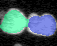
\includegraphics[width=\scalingfactor\textwidth]{images/joint/79_seg_crop.png}}
        };
        \begin{pgfonlayer}{bglower}
            \node[rectangle, color=black,thick, fill=hypothesesbackground!30, opacity=0.8, draw=black,
            fit=(a1) (c2) (a5) (helpercoord1), inner sep=2, opacity=0.8, shift=($(image2) - (image1)$), label={[xshift=15]above:{}}]
            (bglow) {};
        \end{pgfonlayer}
        \begin{pgfonlayer}{lower}
            \begin{scope}[every node/.append style={scale=0.7}]
                \node[fg_det, label={[font=\tiny]center:$X_6^{t+1}$}] (b1) at (image2.south east) {};
                \node[fg_det, label={[font=\tiny]center:$X_7^{t+1}$}] (b2) at (image2.north east) {};
                \node[fg_det, label={[font=\tiny]center:$X_8^{t+1}$}] (b3) at ($(image2.south west)!0.5!(image2.north west)$) {};
            \end{scope}
            \begin{scope}[every node/.append style={scale=0.5}]
                \path[conflict] (b1) edge (b3);
                \path[conflict] (b3) edge (b2);
                \node[conflict] (c1) at ($(b1)!0.5!(b3)$) {};
                \node[conflict] (c2) at ($(b2)!0.5!(b3)$) {};
                \node[count] (c3) at ($(b1)!0.5!(b2)!0.3!(b3)$) {};
                \path[count] (b1) edge (c3);
                \path[count] (b2) edge (c3);
                \path[count] (b3) edge (c3);
            \end{scope}
        \end{pgfonlayer}
    \end{scope}
    \begin{pgfonlayer}{transition}
        \begin{scope}[every node/.append style={scale=0.6}]
            \node[fg_tra,label={[font=\tiny]center:$Y_{1,6}^t$},xshift=30] (trans1) at ($(a1)!0.55!(b1)$) {};
        \end{scope}
        \begin{scope}[every node/.append style={scale=0.2}]
            \node[transfac] (out) at ($(a1.center)!0.5!(trans1)$) {};
            \node[transfac] (in) at ($(b1.center)!0.5!(trans1)$) {};
            \path[transfac] (a1) edge (out.center);
            \path[transfac] (out) edge (trans1);
            \path[transfac] (trans1) edge (in);
            \path[transfac] (in) edge (b1.center);
        \end{scope}
    \end{pgfonlayer}
    \coordinate (base1) at (bglow.north west |- bglow.south west);
    \coordinate (base2) at (bglow.south east |- bglow.south west);
    % \draw [pllbl] (base1) -- (base2) node[black,midway,yshift=-0.6cm] {Factor Graph};
    \path let \p1 = (base1.west), \p2 = (base2.east) in
    node[pllbltxt, minimum width=\x2-\x1] (labelgraph) at ($(base1)!0.5!(base2)$) {Factor Graph};
    \begin{pgfonlayer}{bglower}
        \path[threed] (bglow.south east) -- (bgup.south east);
        \path[threed] (bglow.north east) -- (bgup.north east);
        \path[threed] (bglow.south west) -- (bgup.south west);
        \path[threed] (bglow.north west) -- (bgup.north west);
    \end{pgfonlayer}
\end{scope}

%%% Local Variables: 
%%% mode: latex
%%% TeX-master: "../../../main"
%%% End: 

        % \node[ultra thick, left=of raw1,yshift=5mm] {$t\phantom{+1}$};
        % \node[ultra thick, left=of raw2,yshift=5mm] {$t+1$};
        \begin{scope}[xshift=1.3*\shiftdistance]
    \begin{scope}[yshift=\distancebetween,
        every node/.append style={yslant=0.5,xslant=-1},
        yslant=0.5,xslant=-1]
        \node[inner sep=0, label={[xshift=5]above:{}}] (res1) {
            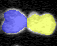
\includegraphics[width=\scalingfactor\textwidth]{images/joint/78_res_crop.png}
        };
    \end{scope}
    \begin{scope}[every node/.append style={yslant=0.5,xslant=-1},yslant=0.5,xslant=-1]
        \begin{pgfonlayer}{bglower}
            \node[inner sep=0, label={[xshift=15]above:{}}] (res2) {
                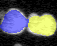
\includegraphics[width=\scalingfactor\textwidth]{images/joint/79_res_crop.png}
            };
        \end{pgfonlayer}
    \end{scope}
    \coordinate (base1) at (res2.north west |- bglow.south west);
    \coordinate (base2) at (res2.south east |- bglow.south west);
    % \draw (base1) rectangle[pllbltxt, yshift=-10] (base2);%  {Tracking Result};
    \path let \p1 = (base1.west), \p2 = (base2.east) in
    node[pllbltxt, minimum width=\x2-\x1]  (labelres) at ($(base1)!0.5!(base2)$) {Tracking Result};
    \begin{pgfonlayer}{bglower}
        \path[threed] (res2.south east) -- (res1.south east);
        \path[threed] (res2.north east) -- (res1.north east);
        \path[threed] (res2.south west) -- (res1.south west);
        \path[threed] (res2.north west) -- (res1.north west);
    \end{pgfonlayer}
\end{scope}

%%% Local Variables: 
%%% mode: latex
%%% TeX-master: "../../../main"
%%% End: 

        \begin{pgfonlayer}{background}
            \node[plbg, fit=(bglow.south west) (bglow.north west)
            (bgup.north east) (res1.south east) (labelres.south)] (bg2) {};
        \end{pgfonlayer}
        \draw[arrows=->, ultra thick, transform canvas={xshift=-15}] (bg2.north west) -- (bg2.south
        west) node[midway, xshift=-7] (t2) {\large{$t$}};
    \end{scope}

    \begin{pgfonlayer}{background}
        \coordinate[xshift=0mm,left=of t1] (hawaii);
        \coordinate[right=of bg1.east,xshift=0mm] (coordeast);
        % \coordinate[below right=of bg1.south east,yshift=-5mm] (coordsouth);
        \coordinate (helper) at ($(bg1.south)!0.5!(bg2.north)$);
        \coordinate (coordsoutheast) at (coordeast |- helper);
        \coordinate[left=of t2.west,xshift=0mm] (coordwestwest);
        \coordinate[xshift=15mm] (coordwest) at (coordwestwest);
        \coordinate (coordsouthwest) at (coordwestwest |- helper);
        \path[arrows=->,draw, line width=4mm, color=red!40, rounded corners=5pt] (hawaii) -- (bg1.east) -- (coordeast) --
(coordsoutheast) -- (coordsouthwest) -- (coordwestwest) -- (coordwest) -- (coordeast |- bg2.east);
    \end{pgfonlayer}
    
\end{tikzpicture}

%%% Local Variables: 
%%% mode: latex
%%% TeX-master: "../../../main"
%%% End: 

        }
        \caption{Joint segmentation and tracking workflow.}
        \label{fig:joint-pipeline}
    \end{figure}
\end{frame}

\begin{frame}
    \frametitle{Definitions}
    \begin{itemize}
          \item \emph{Segment} or \emph{superpixel/-voxel}: Smallest unit in a segmentation
          \item \emph{Region}: Any single segment or union of two neighboring regions
          \item \emph{Conflict}: Two regions that contradict each other
          \item \emph{Connected Component}: A region that has no neighbors (is completely surrounded
        by background)
    \end{itemize}
\end{frame}

\begin{frame}
    \frametitle{Definitions - Example}

\end{frame}

\begin{frame}
    \frametitle{Graphical Model}
    BILD VOM GM
\end{frame}

\begin{frame}
    \frametitle{Graphical Model - Details}
    einige Slides zur Mathematik
\end{frame}

\begin{frame}
    \frametitle{Experiments}
    einige Slides zu den Experimenten
\end{frame}


%%% Local Variables: 
%%% mode: latex
%%% TeX-master: "../main"
%%% End: 
